\documentclass[12pt,openright,oneside,a4paper,english,brazil]{abntex2}

% Pacotes básicos 
\usepackage{lmodern}			% Usa a fonte Latin Modern			
\usepackage[T1]{fontenc}		% Selecao de codigos de fonte.
\usepackage[utf8]{inputenc}		% Codificacao do documento (conversão automática dos acentos)
\usepackage{lastpage}			% Usado pela Ficha catalográfica
\usepackage{indentfirst}		% Indenta o primeiro parágrafo de cada seção.
\usepackage{color}				% Controle das cores
\usepackage{graphicx}			% Inclusão de gráficos
\usepackage{microtype} 			% para melhorias de justificação
\usepackage{amsmath}

% CONFIGURAÇÕES DE PACOTES

% Informações de dados para CAPA e FOLHA DE ROSTO
\titulo{Restauração de Imagens de Placas de Veículos Usando Super-resolução}
\autor{David Campos Anchieta}
\local{Belém - PA}
\data{2017}
\orientador{Prof. Dr. Ronaldo de Freitas Zampolo}
\instituicao{%
	Universidade Federal do Pará
	\par
	Instituto de Tecnologia
	\par
	Faculdade de Engenharia da computação e Telecomunicações}
\tipotrabalho{Trabalho de Conclusão de Curso}
% O preambulo deve conter o tipo do trabalho, o objetivo, 
% o nome da instituição e a área de concentração 

%ISSUE: redigir preambulo
\preambulo{ PREÂMBULO }


% Configurações de aparência do PDF final

% alterando o aspecto da cor azul
\definecolor{blue}{RGB}{41,5,195}

% informações do PDF
\makeatletter
\hypersetup{
			%pagebackref=true,
		pdftitle={\@title}, 
		pdfauthor={\@author},
			pdfsubject={\imprimirpreambulo},
			pdfcreator={LaTeX with abnTeX2},
		pdfkeywords={abnt}{latex}{abntex}{abntex2}{trabalho acadêmico}, 
		colorlinks=true,       		% false: boxed links; true: colored links
			linkcolor=blue,          	% color of internal links
			citecolor=blue,        		% color of links to bibliography
			filecolor=magenta,      		% color of file links
		urlcolor=blue,
		bookmarksdepth=4
}
\makeatother

% Espaçamentos entre linhas e parágrafos 
% O tamanho do parágrafo é dado por:
\setlength{\parindent}{1.3cm}

% Controle do espaçamento entre um parágrafo e outro:
\setlength{\parskip}{0.2cm}  % tente também \onelineskip

% compila o indice
\makeindex

% Início do documento
\begin{document}

% Seleciona o idioma do documento (conforme pacotes do babel)
%\selectlanguage{english}
\selectlanguage{brazil}

% Retira espaço extra obsoleto entre as frases.
\frenchspacing 
% ELEMENTOS PRÉ-TEXTUAIS

% Capa
\imprimircapa

% Folha de rosto
\imprimirfolhaderosto

% Inserir folha de aprovação

% Isto é um exemplo de Folha de aprovação, elemento obrigatório da NBR
% 14724/2011 (seção 4.2.1.3). Você pode utilizar este modelo até a aprovação
% do trabalho. Após isso, substitua todo o conteúdo deste arquivo por uma
% imagem da página assinada pela banca com o comando abaixo:
%
% \includepdf{folhadeaprovacao_final.pdf}
%

\begin{folhadeaprovacao}
%ISSUE: folha de aprovação
	\begin{center}
		{\ABNTEXchapterfont\large\imprimirautor}

		\vspace*{\fill}\vspace*{\fill}
		\begin{center}
			\ABNTEXchapterfont\bfseries\Large\imprimirtitulo
		\end{center}
		\vspace*{\fill}
		
		\hspace{.45\textwidth}
		\begin{minipage}{.5\textwidth}
				\imprimirpreambulo
		\end{minipage}%
		\vspace*{\fill}
	 \end{center}
				
	 Trabalho aprovado. \imprimirlocal, 24 de novembro de 2012:

	 \assinatura{\textbf{\imprimirorientador} \\ Orientador} 
	 \assinatura{\textbf{Professor} \\ Convidado 1}
	 \assinatura{\textbf{Professor} \\ Convidado 2}
	 %\assinatura{\textbf{Professor} \\ Convidado 3}
	 %\assinatura{\textbf{Professor} \\ Convidado 4}
			
	 \begin{center}
		\vspace*{0.5cm}
		{\large\imprimirlocal}
		\par
		{\large\imprimirdata}
		\vspace*{1cm}
	\end{center}
	
\end{folhadeaprovacao}

% Dedicatória
\begin{dedicatoria}
%ISSUE: dedicatória
	 \vspace*{\fill}
	 \centering
	 \noindent
	 \textit{ DEDICATÓRIA} \vspace*{\fill}
\end{dedicatoria}

% Agradecimentos
\begin{agradecimentos}
%ISSUE: agradecimentos


\end{agradecimentos}

% Epígrafe
\begin{epigrafe}
%ISSUE: epígrafe
		\vspace*{\fill}
	\begin{flushright}
		\textit{O que as suas mãos tiverem que fazer,\\
		que o façam com toda a sua força,\\
		pois na sepultura, para onde você vai,\\
		não há atividade nem planejamento,\\
		não há conhecimento nem sabedoria.\\
Eclesiastes 9:10}
	\end{flushright}
\end{epigrafe}

% RESUMOS

% resumo em português
\setlength{\absparsep}{18pt} % ajusta o espaçamento dos parágrafos do resumo
\begin{resumo}
%ISSUE: resumo pt

\end{resumo}

% resumo em inglês
\begin{resumo}[Abstract]
%ISSUE: resumo en
 \begin{otherlanguage*}{english}
	This is the english abstract.

	\vspace{\onelineskip}
 
	\noindent 
	\textbf{Keywords}: latex. abntex. text editoration.
 \end{otherlanguage*}
\end{resumo}


% inserir lista de ilustrações
\pdfbookmark[0]{\listfigurename}{lof}
\listoffigures*
\cleardoublepage
% ---

% ---
% inserir lista de tabelas
% ---
\pdfbookmark[0]{\listtablename}{lot}
\listoftables*
\cleardoublepage
% ---

% ---
% inserir lista de abreviaturas e siglas
% ---
\begin{siglas}
	\item[SR] Super-resolução
	\item[HR] \textit{High resolution} ou alta resolução
\end{siglas}
% ---

% ---
% inserir lista de símbolos
% ---
\begin{simbolos}
%ISSUE: lista de símbolos
	\item[$ \Gamma $] Letra grega Gama
	\item[$ \lambda $] Lambda
	\item[$ \zeta $] Letra grega minúscula zeta
	\item[$ \in $] Pertence
\end{simbolos}
% ---

% ---
% inserir o sumario
% ---
\pdfbookmark[0]{\contentsname}{toc}
\tableofcontents*
\cleardoublepage
% ---



% ----------------------------------------------------------
% ELEMENTOS TEXTUAIS
% ----------------------------------------------------------
\textual

% ----------------------------------------------------------
% Introdução (exemplo de capítulo sem numeração, mas presente no Sumário)
% ----------------------------------------------------------
\chapter[Introdução]{Introdução}
\addcontentsline{toc}{chapter}{Introdução}
% ----------------------------------------------------------
%ISSUE: introdução

\chapter{Restauração de Imagens Usando Super-resolução}
\section{Introdução}
A disponibilidade de um sistema de aquisição de imagens em alta resolução é um aspecto positivo para todas as aplicações que se beneficiam do uso de imagens digitais.
Imagens médicas com boa resolução facilitam o diagnóstico de doenças, por exemplo \cite{park2003super}.
No entanto, gerar imagens de alta resolução pode ter um custo elevado, além de apresentar outros inconvenientes dependendo da aplicação.
Por exemplo, um sistema de vigilância que gerasse imagens de alta resolução precisaria de robustez computacional e alta capacidade de armazenamento para funcionar continuamente.
Sistemas de imagens médicas também enfrentam o dilema de obter imagens melhores sem aumentar a exposição do paciente à radiação \cite{yue2016image}.

Todas essas questões trouxeram a necessidade de técnicas de aprimoramento de imagens que não somente aumentassem a resolução espacial artificialmente, como ocorre em um processo de interpolação, mas que também recuperassem as componentes de alta frequência que se perdem durante o processo de subamostragem.

Entende-se por Super-resolução o processo de obtenção de uma ou mais imagens de alta resolução a partir de uma ou mais imagens de baixa resolução.
Técnicas de super-resolução são estudadas desde os anos 1970 e têm despertado um grande interesse de estudo nas últimas décadas.
As aplicações de técnicas de SR são diversas e incluem aprimoramentos de imagens médicas, de imagens de rosto, de texto e impressões digitais\cite{nasrollahi2014super}.

As abordagens também se diversificaram ao longo dos anos de estudos. Os primeiros algorítimos desenvolvidos faziam o processamento no domínio da frequência, usando transformadas de Fourier e Wavelet.
No entanto, os métodos de SR no domínio da frequência tinham limitações acabaram por ser substituídos por métodos no domínio espacial.



\section{Apreciação das Técnicas de Super-resolução}


\chapter{Super Resolução Bayesiana}
\section{Modelo de Observação}

Definir um modelo de observação que relacione a imagem de alta resolução às imagens de baixa resolução observadas é importante para o desenvolvimento de qualquer técnica de super-resolução.

O modelo de observação deste trabalho tenta simular cinco tipos de alteração aplicadas por sistemas de aquisição de imagens, a saber: rotação, deslocamento, espalhamento de ponto, subamostragem e ruído.
Este modelo de observação é descrito tanto no artigo de Tipping \cite{tipping2003bayesian} quanto em vários outros trabalhos relacionados \cite{pickup2007bayesian}, \cite{Capel01a}.

As alterações de deslocamento linear e rotação tentam simular um possível movimento aleatório na câmera.
A convolução com uma função de espalhamento de ponto Gaussiana repressenta o efeito de falta de foco provocado por uma lente.
A subamostragem simula a baixa densidade de pixels no sensor da câmera,
que seria menor do que a necessária para registrar os dados da imagem acima da taxa de Nyquist.

Pela conveniência do modelo de observação, a imagem de alta resolução de dimensões $m \times n$ é representada por um vetor coluna $\mathbf{x} = [x_1, x_2, ... , x_{N-1}, x_N]^T$ onde $N ={} m \times n$. Ou seja, os valores dos pixels da imagem são rearranjados em um vetor de comprimento $N$.

Sabendo disso, a relação entre uma imagem de alta resolução $\mathbf{x}$ e uma imagem degradada $\mathbf{y}^{(k)}$ é resumida em (\ref{eq:degradation}). Onde $k = 1,2,...,K$; sendo $K$ o número total de quadros obtidos a partir da cena de alta resolução $\mathbf{x}$.

\begin{equation}
	\label{eq:degradation}
	\mathbf{y}^{(k)} = \mathbf{W}^{(k)}\mathbf{x} + \mathbf{n}^{(k)}
\end{equation}

O ruído, representado por $\mathbf{n}$ é um vetor de variáveis aleatórias Gaussianas independentes de média zero e variância $1/\beta$.

A matriz de sistema $\mathbf{W}$ aplica as transformações de rotação, deslocamento, subamostragem e espalhamento de ponto ao ser multiplicada pela imagem de alta resolução $\mathbf{x}$.
Pelas propriedades da multiplicação de matrizes, é natural que as dimensões da matriz do sistema sejam $M \times N$; onde $M$ é o número de pixels da imagem resultante.
Também se espera que $N \gg M$.

A matriz $\mathbf{W}$ depende de três parâmetros de transformação: a largura da função de espalhamento de ponto $\gamma$ um ângulo de rotação $\theta$ e um vetor de deslocamento linear $\mathbf{s}$. Os elementos da matriz são dados por (\ref{eq:wmatrix}) com a função de espalhamento de ponto descrita em (\ref{eq:psf}).

\begin{equation}
	\label{eq:wmatrix}
	W^{(k)}_{ji} = \widetilde{W}^{(k)}_{ji} / \sum_{i'} \widetilde{W}^{(k)}_{ji}
\end{equation}

\begin{equation}
	\label{eq:psf}
	\widetilde{W}^{(k)}_{ji} = \exp \left\{- \frac{\|\mathbf{v}_i - \mathbf{u}^{(k)}_j\|^2}{\gamma^2} \right\}
\end{equation}

Os vetores $\mathbf{u}^{(k)}_j$ representam o centro da função de espalhamento de ponto e é descrito em (\ref{eq:psfcenter}). Caso não houvesse espalhamento de ponto, as coordenadas $\{\mathbf{u}_1, \mathbf{u}_2,\mathbf{u}_3,..., \mathbf{u}_M\}$ seriam os pontos de amostragem da imagem de baixa resolução na imagem de alta resolução. A Figura \ref{fig:transformations} mostra como se dá o processo de subamostragem e outras transformações bidimensionais.

Quando a função de espalhamento de ponto é aplicada, cada pixel da imagem original é uma combinação dos pontos adjacentes.
% O efeito da transformação de espalhamento da função de espalhamento de ponto é o mesmo que o de realizar uma convolução da imagem com uma função Gaussiana bidimensional como a mostrada na Figura \ref{fig:point spread function}

% OBSERVAÇÃO: ADICIONAR FIGURA MOSTRANDO GRÁFICO DA FUNÇÃO DE ESPALHAMENTO DE PONTO

\begin{equation}
	\label{eq:psfcenter}
	\mathbf{u}^{(k)}_j = \mathbf{R}^{(k)}(\mathbf{v}_j-\mathbf{\overline{v}})+\mathbf{\overline{v}}+\mathbf{s}_k
\end{equation}

\begin{equation}
	\mathbf{R}^{(k)} = 
	\begin{pmatrix}
		\cos \theta_k & \sin \theta_k \\
		- \sin \theta_k & \cos \theta_k
	\end{pmatrix}
\end{equation}

\begin{figure}
	\centering
	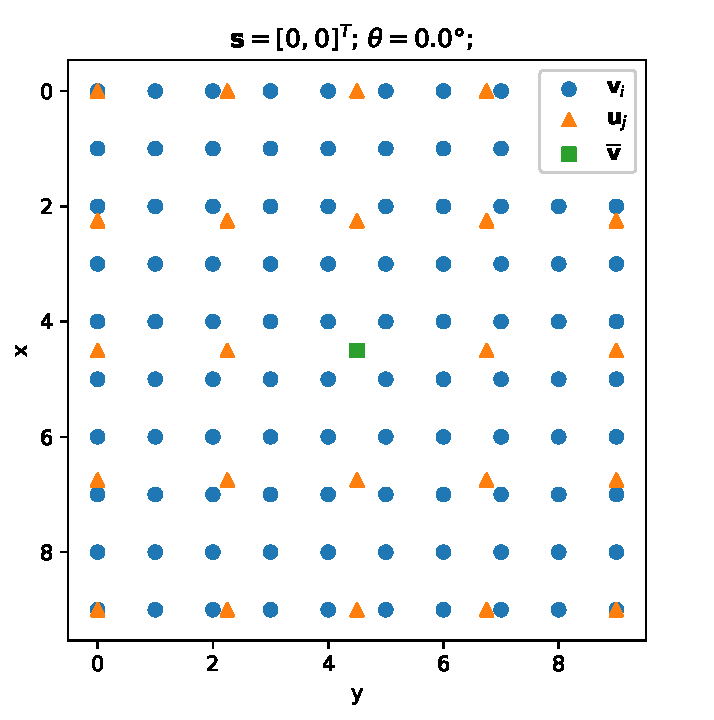
\includegraphics[width=0.4\textwidth]{./figures/transform1.pdf}
	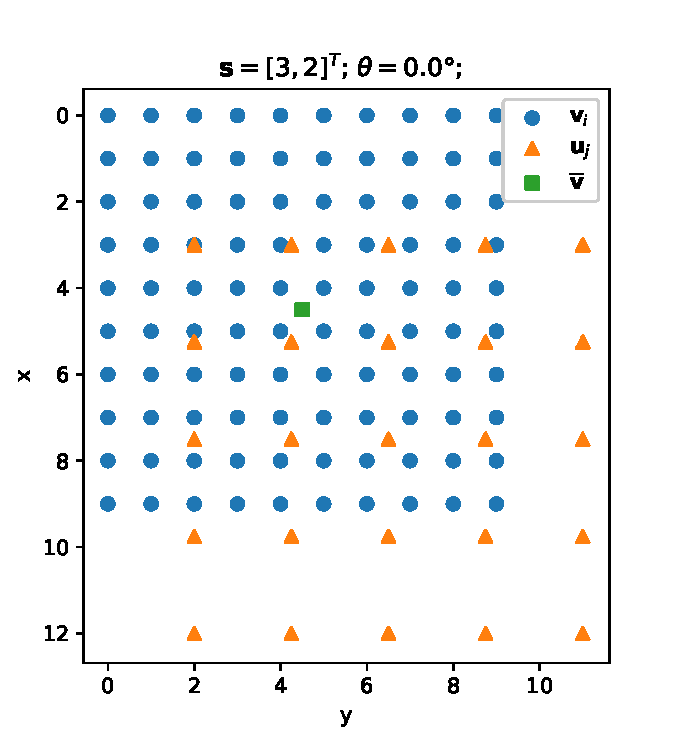
\includegraphics[width=0.4\textwidth]{./figures/transform2.pdf}
	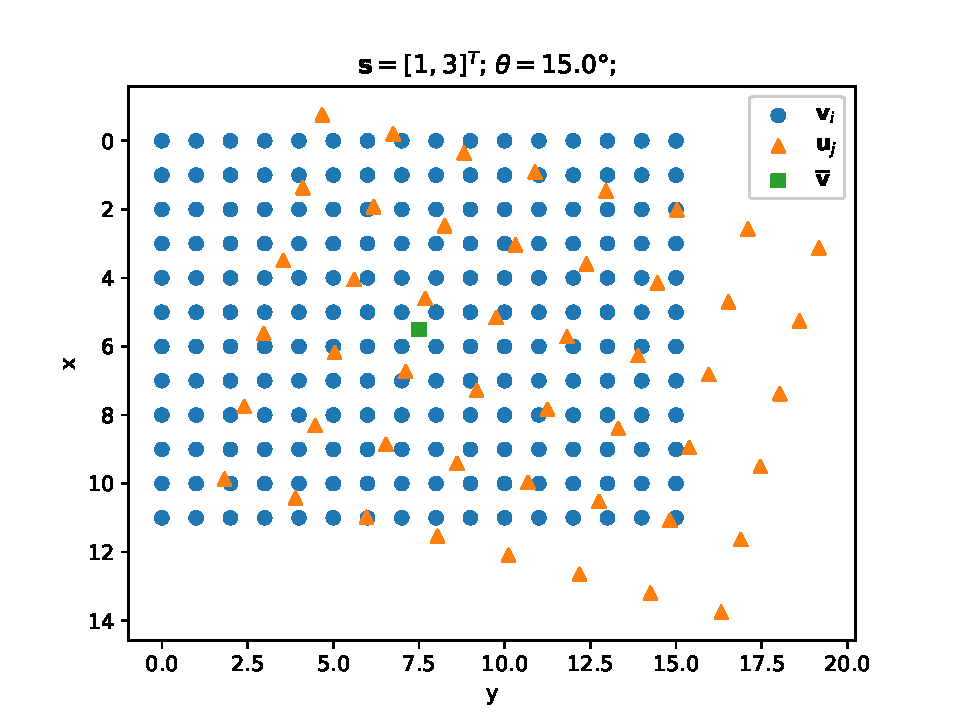
\includegraphics[width=0.4\textwidth]{./figures/transform3.pdf}
	\caption{Visualização das transformações de subamostragem, deslocmento linear e rotação.}
	\label{fig:transformations}
\end{figure}

\chapter{Metodologia}

O método algoritmo por Tipping se vale do método de inferência Bayesiana para obter uma imagem de alta resolução a partir de várias imagens de baixa resolução.
Através de um método de inferência Bayesiana, é possível obter uma estimativa de valores desconhecidos (como a imagem de alta resolução) usando um conhecimento a priori que se tem desses dados e imformações que já estão disponíveis(no caso, as imagens de baixa resolução) \cite{therrien2011probability}.

Sabendo disso, há a necessdade de formular uma distribuição a priori que represente as características estatísticas da imagem que pretendemos estimar a partir dos dados.
A distribuição de probabilidade a priori escolhida para a imagem é uma gaussiana como descrita a seguir:

\begin{gather}
	p(\mathbf{x}) = \mathcal{N}(\mathbf{x} | 0, \mathbf{Z}_x) \\ 
	Z_x(i,j) = A \exp \left\{ - \frac{\|\mathbf{v}_i - \mathbf{v}_j \|^2}{r^2} \right\}
\end{gather}

Onde $A$ é uma constante, e $r$ determina o quanto cada ponto da imagem de alta resolução depende dos pontos vizinhos.
Expandindo a função densidade de probabilidade $p(\mathbf{x})$ temos:

\begin{equation}
	p(\mathbf{x}) = \frac{1}{\sqrt{(2\pi)^N \mathbf{Z}_x}}\exp{-\tfrac{1}{2} \mathbf{x}^T \mathbf{Z}_x \mathbf{x}}
\end{equation}

Este tipo de distribuição não é o ideal, visto que se definirmos $r=1$, estaríamos dizendo que a maioria dos valores dos pontos da imagem de de alta resolução estão contidos no intervalo $[-1,1]$, o que não condiz com a realidade.
No entanto, o uso desta distribuição a priori será mantido no desenvolvimento deste trabalho pela conveniência proporcionada pela função de probabilidade Gaussiana, que facilita algumas manipulações -- como aplicação de logaritmos naturais --  utilizadas a seguir.

Ciente da relação entre a imagem original e as imagens de baixa resolução, podemos escrever a probabilidade a posteriori das imagens de baixa resolução como:

\begin{equation}
	\label{eq:posterior0}
	p(\mathbf{y}^{(k)} | \mathbf{x}, \mathbf{s}_k, \theta_k, \gamma) = 
	\left(\frac{\beta}{2\pi}\right)^{M/2}
	\exp \left\{ -\frac{\beta}{2} \| \mathbf{y}^{(k)} - \mathbf{W}^{(k)} \mathbf{x} \|^2 \right\}.
\end{equation}

Note que esta distribuição é condicionada na imagem de alta resolução e nos parâmetros de degradação, dados que são desconhecidos em um situação real.

Podemos usar o Teorema de Bayes para isolar a imagem original $\mathbf{x}$, ao que obtemos:

\begin{gather}
	\label{eq:posteriordist}
	p(\mathbf{x}|\{\mathbf{y}^{(k)},\mathbf{s}_k,\theta_k\}, \gamma) = 
	\frac{p(\mathbf{x})\prod^K_{k=1} p(\mathbf{y}^{(k)}|\mathbf{x},\mathbf{s}_k,\theta_k, \gamma)}
	{p(\{\mathbf{y}^{(k)}\}|\{\mathbf{s}_k,\mathbf{\theta}_k\},\gamma)} \\
	= \mathcal{N}(\boldsymbol{\mu},\mathbf{\Sigma}) \\
	\mathbf{ \Sigma }= \left[\mathbf{Z}^{-1}_x + \beta \left( \sum^K_{k = 1} \mathbf{W}^{(k)^T} \mathbf{W}^{(k)} \right) \right]^{-1} \\
	\boldsymbol{\mu} = \beta \mathbf{ \Sigma } \left( \sum^K_{k=1} \mathbf{W}^{(k)^T}\mathbf{y}^{(k)} \right).
\end{gather}

Esta função de probabilidade já poderia ser utilizada para inferir a imagem de alta resolução.
Para isso, bastaria encontrar o valor de $\mathbf{x}$ que maximiza o numerador em (\ref{eq:posteriordist}). entretanto, isso exigiria saber os valores dos parâmetros de degradação ($\gamma$, $\theta_k$, $\mathbf{\theta}_k$).
Como esses parâmetros não estão disponíveis, eles também terão de ser estimados a partir das imagens de baixa resolução $\mathbf{y}_k$. 

A solução proposta no artigo é marginalizar $\mathbf{x}$ em (\ref{eq:posterior0}) para que ele não seja mais uma variável na função. O resultado disto é a seguinte distribuição:

\begin{align}
	\label{eq:parameter}
	\log p(\mathrm{y}|\{\mathbf{s}_k,\theta_k\}, \gamma) &= -\frac{1}{2}\left[\beta \sum^K_{k=1} \|\mathbf{y}^{(k)} - \mathbf{W}^{(k)}\boldsymbol{\mu}\|
    + \boldsymbol{\mu}^T\mathbf{Z}_x \boldsymbol{\mu} \right. \nonumber \\
    &\qquad \left.\vphantom{\int_t} + \log |\mathbf{Z}_x| - \log{\Sigma} - KM \log \beta \right].
\end{align}

Onde y é o conjunto de todas as imagens de baixa resolução $\mathbf{y}_k$.

Em uma situação ideal, a melhor estimativa dos valores dos parâmetros de degradação é a que maximiza a função de verossimilhança em (\ref{eq:parameter}).
Tendo a estimativa desses valores, podemos então usá-los em (\ref{eq:posteriordist}) para procurar pelo vetor $\mathbf{x}$ que maximiza aquela função de verossimilhança.

Um fato que se constatou empiricamente na tentativa de calcular os valores da função de verossimilhança é que as probabilidades são muito pequenas ao ponto de estarem fora do intervalo de precisão de uma variável do tipo ponto flutuante.
Os valores também variam muito pouco ao longo do espaço vetorial de $\mathbf{x}$ o que dificultaria o uso de métodos iterativos para encontrar o ponto de máximo da função.

Para resolver isso, aplicou-se o logaritmo natural à função. Isso resolveu o problema da escala e da variação.
Além disso eliminou os exponenciais e os produtos, facilitando o cálculo do gradiente e Jacobiano da função.

\begin{gather}
	L(\mathbf{x}) = -\frac{1}{2} \left\{ \sum^K_{k=1} \|\mathbf{y}^{(k)} - \mathbf{W}^{(k)} \mathbf{x} \|^2 + \mathbf{x}^T\mathbf{Z}^{-1}_x\mathbf{x} - KM\mathrm{ln}(\beta) - \mathrm{ln}|\mathbf{Z}_x| \right\} \\ 
	L'(\mathbf{x}) =  \sum^K_{k=1}  (\mathbf{y}^{(k)} - \mathbf{W}^{(k)}\mathbf{x})(\mathbf{W}^{(k)})^T  - \frac{1}{2}(\mathbf{Z}^{-1}_x + (\mathbf{Z}^{-1}_x)^T)\mathbf{x}  \\
	L''(\mathbf{x}) =  -\sum^K_{k=1} (\mathbf{W}^{(k)})^T\mathbf{W}^{(k)} - \frac{1}{2}(\mathbf{Z}^{-1}_x - (\mathbf{Z}^{-1}_x)^T)^T
\end{gather}


\chapter{Resultados}

\chapter{Conclusão}

% ELEMENTOS PÓS-TEXTUAIS
\postextual

% Referências bibliográficas
\bibliographystyle{plain}
\bibliography{referencias}


\end{document}
